%\documentclass[handout]{beamer}
\documentclass{beamer}

\mode<presentation>
{
%\usetheme{Singapore}
%\usetheme{Warsaw}
\usetheme{Malmoe}
\useinnertheme{circles}
\useoutertheme{infolines}
% \useinnertheme{rounded}

\setbeamercovered{transparent}
}

\usepackage[english]{babel}
\usepackage[latin1]{inputenc}
\usepackage{bm,textpos,alltt,listings,multirow,ulem,minted}
\usepackage{JedMacros}

% font definitions, try \usepackage{ae} instead of the following
% three lines if you don't like this look
\usepackage{mathptmx}
\usepackage[scaled=.90]{helvet}
\usepackage{courier}
\usepackage[T1]{fontenc}
\usepackage{tikz}
\usetikzlibrary[shapes.arrows,arrows,shapes.misc]


\makeatletter
\def\sectionintoc{}
\def\beamer@sectionintoc#1#2#3#4#5{%
\ifnum\c@tocdepth>0%
\ifnum#4=\beamer@showpartnumber%
{
  \beamer@saveanother%
  \gdef\beamer@todo{}%
  \beamer@slideinframe=#1\relax%
  \expandafter\only\beamer@tocsections{\gdef\beamer@todo{%
      \beamer@tempcount=#5\relax%
      \advance\beamer@tempcount by\beamer@sectionadjust%
      \edef\inserttocsectionnumber{\the\beamer@tempcount}%
      \def\inserttocsection{\hyperlink{Navigation#3}{#2}}%
      \beamer@tocifnothide{\ifnum\c@section=#1\beamer@toc@cs\else\beamer@toc@os\fi}%
      {
        \ifbeamer@pausesections\pause\fi%
        \ifx\beamer@toc@ooss\beamer@hidetext
          \vskip.2em
        \else
          \vskip.2em
        \fi
        {%
          \hbox{\vbox{%
              \def\beamer@breakhere{\\}%
              \beamer@tocact{\ifnum\c@section=#1\beamer@toc@cs\else\beamer@toc@os\fi}    {section in toc}}}%
         \par%
        }%
      }%
    }
  }%
  \beamer@restoreanother%
  }
  \beamer@todo%
  \fi\fi%
}
\makeatother


% \usepackage{pgfpages}
% \pgfpagesuselayout{4 on 1}[letterpaper,landscape,border shrink=5mm]

% Macros for the p-Bratu revision numbers
\def\Rbasic{0}
\def\Rrlap{1}
\def\Rrbratu{2}
\def\Rrpbratu{3}
\def\Rassemblebratu{4}
\def\Rassemblepicard{5}
\def\Rmyprealloc{6}
\def\Rnewtoncrash{7}
\def\Rnewtonbug{8}
\def\Rnewtonfix{9}

\title[PETSc]{The Portable Extensible Toolkit for Scientific computing}

\author{Barry Smith}


% - Use the \inst command only if there are several affiliations.
% - Keep it simple, no one is interested in your street address.
\institute[ANL]{Mathematics and Computer Science Division, Argonne National Laboratory}

\date{ATPESC 2013-08-02}


% This is only inserted into the PDF information catalog. Can be left
% out.
\subject{Talks}



% If you have a file called "university-logo-filename.xxx", where xxx
% is a graphic format that can be processed by latex or pdflatex,
% resp., then you can add a logo as follows:

% \pgfdeclareimage[height=0.5cm]{university-logo}{university-logo-filename}
% \logo{\pgfuseimage{university-logo}}



% Delete this, if you do not want the table of contents to pop up at
% the beginning of each subsection:
\AtBeginSubsection[]
{
 \begin{frame}<beamer>
 \frametitle{Outline}
 \tableofcontents[currentsection,currentsubsection]
 \end{frame}
}

\AtBeginSection[]{
\begin{frame}<beamer>
  \frametitle{Outline}
  \tableofcontents[currentsection]
\end{frame}
}

% If you wish to uncover everything in a step-wise fashion, uncomment
% the following command:

%\beamerdefaultoverlayspecification{<+->}

\begin{document}
\lstset{language=C}

\begin{frame}
\titlepage
Thanks to Jed Brown and Matt Knepley for the slides
\end{frame}

\begin{frame}
\frametitle{Outline}
\tableofcontents
% You might wish to add the option [pausesections]
\end{frame}
\begin{frame}{Follow Up; Getting Help}
  \begin{itemize}
    \item \url{http://www.mcs.anl.gov/petsc}
    \item Public questions: \url{petsc-users@mcs.anl.gov}, archived
    \item Private questions: \url{petsc-maint@mcs.anl.gov}, not archived
  \end{itemize}
\end{frame}


\section{Introduction}
\newcommand\ganttline[4]{% line, tag, start end
   \node at (0,#1*0.4+.1) [anchor=base east] {#2};
   \fill[blue] (#3/\xtick-1991/\xtick,#1*0.4-.1) rectangle (#4/\xtick-1991/\xtick,#1*0.4+.1);}
\newcommand\ganttlabel[6]{% year, label, color, yloc, anchor
  \node[#3] at (#1/\xtick+#6/\xtick-1991/\xtick,#4) [anchor=#5] {#2};
  \fill[#3] (#1/\xtick-1991/\xtick,1/2-.1) rectangle (#1/\xtick-1991/\xtick+0.04,12/2+.1);}

%\begin{frame}{Timeline}
\frame{
\begin{figure}[htbp]
\def\present{2014.9}
\def\xtick{2.2}
\begin{tikzpicture}[y=-1cm]
   %\draw[help lines] (0.5,5) grid (8,0.5);
   \ganttlabel{1991}{1991}{red}{6.2}{north}{0}
   \ganttlabel{1995}{1995}{red}{6.2}{north}{0}
   \ganttlabel{2000}{2000}{red}{6.2}{north}{0}
   \ganttlabel{2005}{2005}{red}{6.2}{north}{0}
   \ganttlabel{2010}{2010}{red}{6.2}{north}{0}
   \ganttlabel{1992}{PETSc-1}{green!70!black}{0}{center}{0}
   \ganttlabel{1994.4}{MPI-1}{magenta!70!black}{-.5}{center}{0}
   \ganttlabel{1997.6}{MPI-2}{magenta!70!black}{-.5}{center}{0}
   \ganttlabel{1995.5}{PETSc-2}{green!70!black}{0}{center}{0}
   \ganttlabel{2008.9}{PETSc-3}{green!70!black}{0}{center}{0}
   \ganttline{1}{Barry}{1991}{\present}
   \ganttline{2}{Bill}{1991}{1996}
   \ganttline{3}{Lois}{1993}{2001}
   \ganttline{4}{Satish}{1997}{\present}
   \ganttline{5}{Dinesh}{1998}{2005.5}
   \ganttline{6}{Hong}{2001}{\present}
   \ganttline{7}{Kris}{2001}{2006}
   \ganttline{8}{Matt}{2001.5}{\present}
   \ganttline{9}{Victor}{2003}{2006.9}
   \ganttline{9}{}{2007.3}{2007.5}
   \ganttline{9}{}{2008.5}{2008.7}
   \ganttline{10}{Dmitry}{2005.6}{\present}
   \ganttline{11}{Lisandro}{2006.9}{\present}
   \ganttline{12}{Jed}{2009}{\present}
   \ganttline{13}{Shri}{2009.8}{\present}
   \ganttline{14}{Peter}{2011.6}{2014.5}
   \ganttline{15}{Mark}{2011.9}{\present}
\end{tikzpicture}
\end{figure}
}
%\end{frame}

\begin{frame}{Commits to the PETSc Repository}

\begin{center}
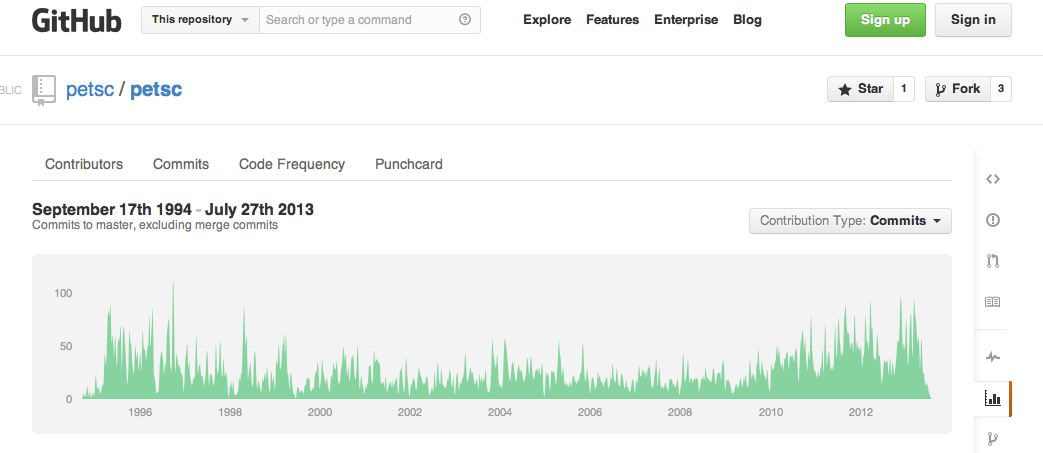
\includegraphics[width=5.0in]{figures/PETSc/Commits}
\end{center}

\end{frame}

\begin{frame}{{\bf Portable} Extensible Toolkit for Scientific computing}
%TODO: big-iron image
\begin{itemize}
  \item Architecture
    \begin{itemize}
    \item tightly coupled (e.g. Cray, Blue Gene)
    \item loosely coupled such as network of workstations
    \item GPU clusters (many vector and sparse matrix kernels)
    \end{itemize}
  \item Operating systems (Linux, Mac, Windows, BSD, proprietary Unix)
  \item Any compiler
  \item Real/complex, single/double/quad precision, 32/64-bit int
  \item Usable from C, C++, Fortran 77/90, Python, and MATLAB
  \item Free to everyone (2-clause BSD license), open development
  \item $10^{12}$ unknowns, full-machine scalability on Top-10 systems \\
  \item Same code runs performantly on a laptop
  \item<2> \alert{\tikz[baseline] \node [cross out,draw=black,line width=1,anchor=text] {No}; iPhone support}
\end{itemize}
\end{frame}

\begin{frame}{Portable {\bf Extensible} Toolkit for Scientific computing}
\begin{block}{Philosophy: Everything has a plugin architecture}
\begin{itemize}
  \item Vectors, Matrices, Coloring/ordering/partitioning algorithms
  \item Preconditioners, Krylov accelerators
  \item Nonlinear solvers, Time integrators
  \item Spatial discretizations/topology$^*$
\end{itemize}
\end{block}
\begin{example}
	Vendor supplies matrix format and associated preconditioner, distributes
	compiled shared library.  Application user loads plugin at runtime, no source
	code in sight.
\end{example}
\end{frame}

\begin{frame}{Portable Extensible {\bf Toolkit} for Scientific computing}
Algorithms, (parallel) debugging aids, low-overhead profiling
\begin{block}{Composability}
Try new algorithms by choosing from product space and composing
existing algorithms (multilevel, domain decomposition, splitting).
\end{block}
\begin{block}{Experimentation}
\begin{itemize}
  \item It is not possible to pick the solver \emph{a priori}. \\
  What will deliver best/competitive performance for a given physics, discretization, architecture, and problem size?
  \item PETSc's response: expose an algebra of composition so new solvers can be created at runtime.
  \item Important to keep solvers decoupled from physics and discretization because we also experiment with those. 
\end{itemize}
\end{block}
\end{frame}

\begin{frame}{Portable Extensible Toolkit for {\bf Scientific computing}}
  \begin{itemize}
  \item Computational Scientists
    \begin{itemize}
    \item PyLith (CIG), Underworld (Monash), Climate (ICL/UK Met), PFLOTRAN (DOE), MOOSE (DOE), Proteus (ERDC)
    \end{itemize}
  \item Algorithm Developers (iterative methods and preconditioning)
  \item Package Developers
    \begin{itemize}
    \item SLEPc, TAO, Deal.II, Libmesh, FEniCS, PETSc-FEM, MagPar, OOFEM, FreeCFD, OpenFVM
    \end{itemize}
  \item Funding
    \begin{itemize}\item Department of Energy
      \begin{itemize}\item SciDAC, ASCR ISICLES, MICS Program, INL Reactor Program
      \end{itemize}
    \item National Science Foundation
      \begin{itemize}\item CIG, CISE, Multidisciplinary Challenge Program
      \end{itemize}
    \end{itemize}
  \item Hundreds of tutorial-style examples
  \item Hyperlinked manual, examples, and manual pages for all routines
  \item Support from \url{petsc-maint@mcs.anl.gov}
  %\item Mailing list \url{petsc-users@mcs.anl.gov}
\end{itemize}
\end{frame}

\input{slides/PETSc/RoleOfPETSc.tex}


\begin{frame}{Better To Use than PETSc}
 Use the package with the highest level of abstraction that uses PETSc

    \begin{itemize}
    \item Eigenvalues - SLEPc,
    \item Optimizationation (with PDE constraints) - TAO
    \item Finite Elements -  Deal.II, Libmesh, FEniCS, PETSc-FEM,  OOFEM, 
    \item Finite Elements and Multiphysics - MOOSE 
    \item Finite Volumes -  FreeCFD, OpenFVM
    \item Wave Propagation - PyClaw
    \item Micromagnetics - MagPar
    \end{itemize}
\end{frame}





\begin{frame}{Advice from Bill Gropp}
  \begin{quote}\large
    You want to think about how you decompose your data structures, how
    you think about them globally.  [...]  If you were building a house,
    you'd start with a set of blueprints that give you a picture of what
    the whole house looks like.  You wouldn't start with a bunch of
    tiles and say. ``Well I'll put this tile down on the ground, and
    then I'll find a tile to go next to it.''  But all too many people
    try to build their parallel programs by creating the smallest
    possible tiles and then trying to have the structure of their code
    emerge from the chaos of all these little pieces.  You have to have
    an organizing principle if you're going to survive making your code
    parallel.
  \end{quote}
  {\small \centering (\url{http://www.rce-cast.com/Podcast/rce-28-mpich2.html})}
\end{frame}


\input{slides/PETSc/PETScPyramid.tex}

\section{Objects - Building Blocks of the Code}


\begin{frame}{MPI communicators}
  \begin{itemize}
  \item Opaque object, defines process group and synchronization channel
  \item PETSc objects need an \code{MPI\_Comm} in their constructor
    \begin{itemize}
    \item \code{PETSC\_COMM\_SELF} for serial objects
    \item \code{PETSC\_COMM\_WORLD} common, but \emph{not} required
    \end{itemize}
  \item Can split communicators, spawn processes on new communicators, etc
  \item Operations are one of
    \begin{itemize}
    \item Not Collective: \code{VecGetLocalSize(), MatSetValues()}
    \item Logically Collective: \code{KSPSetType(), PCMGSetCycleType()}
      \begin{itemize}
      \item checked when running in debug mode
      \end{itemize}
    \item Neighbor-wise Collective: \code{VecScatterBegin(), MatMult()}
      \begin{itemize}
      \item Point-to-point communication between two processes
      \item Neighbor collectives in upcoming MPI-3
      \end{itemize}
    \item Collective: \code{VecNorm(), MatAssemblyBegin(), KSPCreate()}
      \begin{itemize}
      \item Global communication, synchronous
      \item Non-blocking collectives in upcoming MPI-3
      \end{itemize}
    \end{itemize}
  \item Deadlock if some process doesn't participate (\eg wrong order)
  \end{itemize}
\end{frame}




\begin{frame}[fragile]{Objects}
  % \begin{lstlisting}
  %   Mat A;
  %   PetscInt m,n,M,N;
  %   MatCreate(comm,&A);
  %   MatSetSizes(A,m,n,M,N);      /* or PETSC_DECIDE */ 
  %   MatSetOptionsPrefix(A,"foo_");
  %   MatSetFromOptions(A);
  %   /* Use A */
  %   MatView(A,PETSC_VIEWER_DRAW_WORLD);
  %   MatDestroy(A);
  % \end{lstlisting}
  \begin{minted}{c}
    Mat A;
    PetscInt m,n,M,N;
    MatCreate(comm,&A);
    MatSetSizes(A,m,n,M,N);      /* or PETSC_DECIDE */ 
    MatSetOptionsPrefix(A,"foo_");
    MatSetFromOptions(A);
    /* Use A */
    MatView(A,PETSC_VIEWER_DRAW_WORLD);
    MatDestroy(A);
  \end{minted}
  \begin{itemize}
  \item \code{Mat} is an opaque object (pointer to incomplete type)
    \oneitem{Assignment, comparison, etc, are cheap}
  \item What's up with this ``Options'' stuff?
    \begin{itemize}
    \item Allows the type to be determined at runtime: \code{-foo\_mat\_type sbaij}
    \item Inversion of Control similar to ``service locator'', \\
      related to ``dependency injection''
    \item Other options (performance and semantics) can be changed at
      runtime under \code{-foo\_mat\_}
    \end{itemize}
  \end{itemize}
\end{frame}

\input{slides/PETSc/PetscObject.tex}

\section{Options Database - Controling the Code}
\begin{frame}{Ways to set options}
  \begin{itemize}
  \item Command line
  \item Filename in the third argument of \code{PetscInitialize()}
  \item \code{$\sim$/.petscrc}
  \item \code{\$PWD/.petscrc}
  \item \code{\$PWD/petscrc}
  \item \code{PetscOptionsInsertFile()}
  \item \code{PetscOptionsInsertString()}
  \item \code{PETSC\_OPTIONS} environment variable
  \item command line option \code{-options\_file [file]}
  \end{itemize}
\end{frame}

\begin{frame}{Try it out}
  \shell{\small cd \$PETSC\_DIR/src/snes/examples/tutorials \&\& make ex5} \\
  \begin{itemize}
  \item \shell{./ex5 -da\_grid\_x 10 -da\_grid\_y 10 -par 6.7 \\
      -snes\_monitor -\{ksp,snes\}\_converged\_reason \\
      -snes\_view}
  \item \shell{./ex5 -da\_grid\_x 10 -da\_grid\_y 10 -par 6.7 \\
      -snes\_monitor -\{ksp,snes\}\_converged\_reason \\
      -snes\_view -mat\_view draw -draw\_pause 0.5}
  \item \shell{./ex5 -da\_grid\_x 10 -da\_grid\_y 10 -par 6.7 \\
      -snes\_monitor -\{ksp,snes\}\_converged\_reason \\
      -snes\_view -mat\_view draw -draw\_pause 0.5 \\
      -pc\_type lu -pc\_factor\_mat\_ordering\_type natural}
  \item Use \code{-help} to find other ordering types
\end{itemize}
\end{frame}

\begin{frame}[fragile]{Sample output}
\begin{Verbatim}[formatcom=\footnotesize]
  0 SNES Function norm 1.139460779565e+00 
  Linear solve converged due to CONVERGED_RTOL iterations 1
  1 SNES Function norm 4.144493702305e-02 
  Linear solve converged due to CONVERGED_RTOL iterations 1
  2 SNES Function norm 6.309075568032e-03 
  Linear solve converged due to CONVERGED_RTOL iterations 1
  3 SNES Function norm 3.359792279909e-04 
  Linear solve converged due to CONVERGED_RTOL iterations 1
  4 SNES Function norm 1.198827244256e-06 
  Linear solve converged due to CONVERGED_RTOL iterations 1
  5 SNES Function norm 1.545029314765e-11 
\end{Verbatim}
\vspace{-1em}
\includegraphics[width=0.5\textwidth]{figures/Ex5NaturalFill}
\includegraphics[width=0.5\textwidth]{figures/Ex5NDFill}
\end{frame}

\begin{frame}[fragile]{Sample output (SNES and KSP)}
\begin{Verbatim}[formatcom=\footnotesize]
SNES Object: 1 MPI processes
  type: ls
    line search variant: CUBIC
    alpha=1.000000000000e-04, maxstep=1.000000000000e+08, minlambda=1.000000000000e-12
    damping factor=1.000000000000e+00
  maximum iterations=50, maximum function evaluations=10000
  tolerances: relative=1e-08, absolute=1e-50, solution=1e-08
  total number of linear solver iterations=5
  total number of function evaluations=6
  KSP Object:   1 MPI processes
    type: gmres
      GMRES: restart=30, using Classical (unmodified) Gram-Schmidt Orthogonalization with no iterative refinement
      GMRES: happy breakdown tolerance 1e-30
    maximum iterations=10000, initial guess is zero
    tolerances:  relative=1e-05, absolute=1e-50, divergence=10000
    left preconditioning
    using PRECONDITIONED norm type for convergence test
\end{Verbatim}
\end{frame}
\begin{frame}[fragile]{Sample output (PC and Mat)}
\begin{Verbatim}[formatcom=\footnotesize]
  PC Object:   1 MPI processes
    type: lu
      LU: out-of-place factorization
      tolerance for zero pivot 2.22045e-14
      matrix ordering: nd
      factor fill ratio given 5, needed 2.95217
        Factored matrix follows:
          Matrix Object:           1 MPI processes
            type: seqaij
            rows=100, cols=100
            package used to perform factorization: petsc
            total: nonzeros=1358, allocated nonzeros=1358
            total number of mallocs used during MatSetValues calls =0
              not using I-node routines
    linear system matrix = precond matrix:
    Matrix Object:     1 MPI processes
      type: seqaij
      rows=100, cols=100
      total: nonzeros=460, allocated nonzeros=460
      total number of mallocs used during MatSetValues calls =0
        not using I-node routines
\end{Verbatim}
\end{frame}

\begin{frame}{In parallel}
  \begin{itemize}
  \item \shell{mpiexec -n 4 \\
      ./ex5 -da\_grid\_x 10 -da\_grid\_y 10 -par 6.7 \\
      -snes\_monitor -\{ksp,snes\}\_converged\_reason \\
      -snes\_view -sub\_pc\_type lu}
  \item How does the performance change as you
    \begin{itemize}
    \item vary the number of processes (up to 32 or 64)?
    \item increase the problem size?
    \item use an inexact subdomain solve?
    \item try an overlapping method: \code{-pc\_type asm -pc\_asm\_overlap 2}
    \item simulate a big machine: \code{-pc\_asm\_blocks 512}
    \item change the Krylov method: \code{-ksp\_type ibcgs}
    \item use algebraic multigrid: \code{-pc\_type hypre}
    \item use smoothed aggregation multigrid: \code{-pc\_type ml}
    \end{itemize}
  \end{itemize}
\end{frame}


\section[Core/Algorithms]{Core PETSc Components and Algorithms Primer}
\subsection{Time integration}
\begin{frame}{IMEX time integration in PETSc}
  \begin{itemize}
  \item Additive Runge-Kutta IMEX methods
    \begin{gather*}
      G(t,x,\dot x) = F(t,x) \\
      J_\alpha = \alpha G_{\dot x} + G_x
    \end{gather*}
    \vspace{-1em}
    \begin{itemize}
    \item User provides:
      \begin{itemize}
      \item \texttt{FormRHSFunction(ts,$t$,$x$,$F$,void *ctx);}
      \item \texttt{FormIFunction(ts,$t$,$x$,$\dot x$,$G$,void *ctx);}
      \item \texttt{FormIJacobian(ts,$t$,$x$,$\dot x$,$\alpha$,$J$,$J_{p}$,mstr,void *ctx);}
      \end{itemize}
    \item Can have $L$-stable DIRK for stiff part $G$, SSP explicit part, etc.
    \item Orders 2 through 5, embedded error estimates
    \item Dense output, hot starts for Newton
    \item More accurate methods if $G$ is linear, also Rosenbrock-W
    \item Can use preconditioner from classical ``semi-implicit'' methods
    \item FAS nonlinear solves supported
    \item Extensible adaptive controllers, can change order within a family
    \item Easy to register new methods: \code{TSARKIMEXRegister()}
    \end{itemize}
  \item Single step interface so user can have own time loop
  \item Same interface for Extrapolation IMEX, LMS IMEX (in development)
  \end{itemize}
\end{frame}

\input{slides/SNES/FlowControl.tex}
\input{slides/PETSc/TSMethods.tex}
\begin{frame}{TS Examples}
  \begin{itemize}
  \item 1D nonlinear hyperbolic conservation laws
    \begin{itemize}
    \item \code{src/ts/examples/tutorials/ex9.c}
    \item {\footnotesize \code{./ex9 -da\_grid\_x 100 -initial 1 -physics shallow -limit minmod -ts\_ssp\_type rks2 -ts\_ssp\_nstages 8 -ts\_monitor\_draw\_solution}}
    \end{itemize}
  \item Stiff linear advection-reaction test problem
    \begin{itemize}
    \item \code{src/ts/examples/tutorials/ex22.c}
    \item {\footnotesize \code{./ex22 -da\_grid\_x 200 -ts\_monitor\_draw\_solution -ts\_type rosw -ts\_rosw\_type ra34pw2 -ts\_adapt\_monitor}}
    \end{itemize}
  \item 1D Brusselator (reaction-diffusion)
    \begin{itemize}
    \item \code{src/ts/examples/tutorials/ex25.c}
    \item {\footnotesize \code{./ex25 -da\_grid\_x 40 -ts\_monitor\_draw\_solution -ts\_type rosw -ts\_rosw\_type 2p -ts\_adapt\_monitor}}
    \end{itemize}
  \end{itemize}
\end{frame}


\subsection{Nonlinear solvers: SNES}
\begin{frame}{Newton iteration: workhorse of SNES}
  \begin{textblock}{3}(11,0)
    \includegraphics[width=\textwidth]{figures/Newton}
  \end{textblock}
  \begin{itemize}
  \item Standard form of a nonlinear system
    \[ F(u) = 0 \]
  \item Iteration
    \begin{align*}
      \text{Solve:} & \qquad J(u) w = -F(u) \\
      \text{Update:} & \qquad u^+ \gets u + w
    \end{align*}
    \item Quadratically convergent near a root: $\abs{u^{n+1}-u^*} \in \bigO\Big(\abs{u^n-u^*}^2\Big)$
    \item Picard is the same operation with a different $J(u)$
  \end{itemize}
  \begin{example}[Nonlinear Poisson]
    \begin{align*}
      F(u)=0 \quad &\sim\quad -\div\big[ (1+u^2) \nabla u \big] - f = 0 \\
      J(u)w \quad &\sim\quad  -\div\big[(1+u^2)\nabla w + 2uw\nabla u \Big]
    \end{align*}
  \end{example}
  % \begin{example}[$\pp$-Bratu]
  %   Suppose $F$ is a discretization of
  %   \[ -\nabla \cdot \big( \eta \nabla u \big) - \lambda e^u - f = 0 \]
  %   \[\eta(\gamma) = (\epsilon^2+\gamma)^{\frac{\pfrak-2}{2}}, \qquad\quad \gamma = \half \abs{\nabla u}^2. \]
  %   Then $J(u)w$ is a discretization of
  %   \[ -\nabla \cdot \big( \eta \nabla w + \eta' (\nabla u \cdot \nabla w)\nabla u \big) - \lambda e^{u} w . \]
  % \end{example}
\end{frame}


\input{slides/SNES/Callbacks.tex}
\input{slides/SNES/Function.tex}
\input{slides/SNES/Jacobian.tex}


\subsection{Linear Algebra background/theory}
\input{slides/MatrixDefinition.tex}
\input{slides/MatricesImportant.tex}
\input{slides/MatrixNoEntries.tex}
\input{slides/GMRES.tex}

\subsection{Structured grid distribution: DMDA}

\begin{frame}{Distributed Array}
  \begin{itemize}
  \item Interface for topologically structured grids
  \item Defines (topological part of) a finite-dimensional function space
    \oneitem{Get an element from this space: \code{DMCreateGlobalVector()}}
  \item Provides parallel layout
  \item Refinement and coarsening
    \oneitem{\code{DMRefineHierarchy()}}
  \item Ghost value coherence
    \oneitem{\code{DMGlobalToLocalBegin()}}
  \item Matrix preallocation: \oneitem{\code{DMCreateMatrix()} (formerly \code{DMGetMatrix()})}
  \end{itemize}
\end{frame}

\input{slides/DA/GhostValues.tex}
\input{slides/DA/GlobalNumberings.tex}
\input{slides/DA/LocalNumbering.tex}
\input{slides/DA/Vectors.tex}
\input{slides/DA/UpdatingGhosts.tex}
\input{slides/DA/Stencils.tex}
\input{slides/DA/CreatingDA2d.tex}
\input{slides/DA/WorkingWithLocal.tex}
\input{slides/DA/LocalFunction.tex}
\input{slides/DA/BratuResidual.tex}

\begin{frame}{Other DMs}
  \begin{itemize}
  \item DMPlex - sophisticated dimension-independent management of unstructured meshes as a CW complex
  \item DMNetwork - for discrete networks like power grids and circuits
  \item DMMoab - interface to the MOAB unstructured mesh library
  \end{itemize}
\end{frame}


\subsection{Profiling}
\input{slides/PETSc/Integration/Profiling.tex}
\input{slides/ReadingLogSummary.tex}
\input{slides/CommunicationCosts.tex}

\subsection{Matrix Redux}
\input{slides/PETSc/Integration/MatrixRedux.tex}
\input{slides/PETSc/Integration/MatrixCreation.tex}
\input{slides/PETSc/Integration/MatrixPolymorphism.tex}
\input{slides/PETSc/Integration/MatrixAssembly.tex}
\input{slides/PETSc/Integration/MisguidedMatrixAssembly.tex}
\input{slides/PETSc/Integration/EfficientMatrixAssembly.tex}
\input{slides/PETSc/Integration/WhyArePETScMatricesThatWay.tex}

\section*{Preliminary Conclusions}
\begin{frame}{Preliminary Conclusions}
  \begin{block}{PETSc can help you}
    \begin{itemize}
    \item solve algebraic and DAE problems in your application area
    \item rapidly develop efficient parallel code, can start from examples
    \item develop new solution methods and data structures
    \item debug and analyze performance
    \item advice on software design, solution algorithms, and performance
      \begin{itemize}
        \item Public questions: \url{petsc-users@mcs.anl.gov}, archived
        \item Private questions: \url{petsc-maint@mcs.anl.gov}, not archived
      \end{itemize}
    \end{itemize}
  \end{block}
  \begin{block}{You can help PETSc}
    \begin{itemize}
    \item report bugs and inconsistencies, or if you think there is a better way
    \item tell us if the documentation is inconsistent or unclear
    \item consider developing new algebraic methods as plugins, contribute if your idea works
    \end{itemize}
  \end{block}
\end{frame}


\part{Integration and Efficiency}
\section{Application Integration}
\input{slides/PETSc/Integration/ApplicationIntegration.tex}
\input{slides/ApplicationIntegration.tex}
\input{slides/PETSc/Integration/Stages.tex}
\input{slides/PETSc/Integration/Initialization.tex}
\input{slides/PETSc/MatrixMemoryPreallocation.tex}
\input{slides/PETSc/Integration/LinearSolvers.tex}
\input{slides/PETSc/Integration/NonlinearSolvers.tex}

\section{Performance and Scalability}
\input{slides/JFNKBottlenecks.tex}
\input{slides/ScalabilityDefinition.tex}
\begin{frame}{Scalability Warning}
  \begin{quote}\Large \centering
    The easiest way to make software scalable \\
    is to make it sequentially inefficient. \\
    (Gropp 1999)
  \end{quote}

  \begin{itemize}
  \item We really want \emph{efficient} software
  \item Need a performance model
    \begin{itemize}
    \item memory bandwidth and latency
    \item algorithmically critical operations (\eg dot products, scatters)
    \item floating point unit
    \end{itemize}
  \item Scalability shows marginal benefit of adding more cores, nothing more
  \item Constants hidden in the choice of algorithm
  \item Constants hidden in implementation
  \end{itemize}
\end{frame}

\subsection{Memory hierarchy}
\input{slides/CPUArchitecture.tex}
\input{slides/HardwareCapability.tex}
\input{slides/OlikerSpMVOptimization.tex}
\input{slides/SpMVPerformanceModel.tex}
\input{slides/StreamTriad-XT5-BGP.tex}
\begin{frame}{Optimizing Sparse Mat-Vec}
  \begin{itemize}
  \item Order unknowns so vector reuses cache (Cuthill-McKee)
    \begin{itemize}
    \item Optimal: $\frac{(2 \text{ flops})(\text{bandwidth})}{\texttt{sizeof(Scalar)} + \texttt{sizeof(Int)}}$
    \item Usually improves strength of ILU and SOR
    \end{itemize}
  \item Coalesce indices for adjacent rows (Inodes)
    \begin{itemize}
    \item Optimal: $\frac{(2 \text{ flops})(\text{bandwidth})}{\texttt{sizeof(Scalar)} + \texttt{sizeof(Int)}/i}$
    \item Can do block SOR (much stronger than scalar SOR)
    \item Default in PETSc, turn off with \code{-mat\_no\_inode}
    \item Requires ordering unknowns so that fields are interlaced, this
      is (much) better for memory use anyway
    \end{itemize}
  \item Use explicit blocking, hold one index per block (BAIJ format)
    \begin{itemize}
    \item Optimal: $\frac{(2 \text{ flops})(\text{bandwidth})}{\texttt{sizeof(Scalar)} + \texttt{sizeof(Int)}/b^2}$
    \item Block SOR and factorization
    \item Symbolic factorization works with blocks (much cheaper)
    \item Very regular memory access, unrolled dense kernels
    \item Faster insertion: \code{MatSetValuesBlocked()}
    \end{itemize}
  \end{itemize}
\end{frame}

\begin{frame}[shrink=5]{Performance of assembled versus unassembled}
  \vspace{1ex}
  \includegraphics[width=\textwidth]{figures/TensorVsAssembly} \\
  \begin{itemize}
  \item Arithmetic intensity for $\Qk p$ elements
    \begin{itemize}
    \item $< \frac 1 4$ (assembled), $\approx 10$ (unassembled), $\approx 4$ to $8$ (hardware)
    \end{itemize}
  \item store Jacobian information at Quass quadrature points, can use AD
  \end{itemize}
\end{frame}

\input{slides/OptimizingSpMVUnassembled.tex}
\begin{frame}{Hardware Arithmetic Intensity}
  \begin{tabular}{lc}
    \toprule
    Operation                         & Arithmetic Intensity (flops/B) \\
    \midrule
    Sparse matrix-vector product      & 1/6                  \\
    Dense matrix-vector product       & 1/4                  \\
    Unassembled matrix-vector product, residual & $\gtrsim 8$          \\
    %High-order residual evaluation    & $\gtrsim 5$                \\
    \bottomrule
  \end{tabular}

  \bigskip

  \begin{tabular}{lrrr}
    \toprule
    Processor & \textsc{stream} Triad (GB/s) & Peak (GF/s) & Balance (F/B) \\
    \midrule
    E5-2680 8-core      & 38   & 173  & 4.5 \\ % http://www.cs.virginia.edu/stream/stream_mail/2013/0001.html
    E5-2695v2 12-core & 45 & 230 & 5.2 \\ % Edison 460 GF and 89 GB/s Triad
    E5-2699v3 18-core & 60 & 660 & 11 \\
    % Magny Cours 16-core & 49   & 281  & 5.7 \\
    Blue Gene/Q node    & 29.3   & 205  & 7 \\ % Morozov's best Triad (https://hpgmg.org/lists/archives/hpgmg-forum/2014-June/000071.html)
    % Tesla M2090         & 120  & 665  & 5.5 \\
    Kepler K20Xm        & 160 & 1310 & 8.2 \\ % http://www.elekslabs.com/2012/11/nvidia-tesla-k20-benchmark-facts.html
    Xeon Phi SE10P      & 161 & 1060 & 6.6 \\ % http://www.cs.virginia.edu/stream/stream_mail/2013/0002.html
    % http://blogs.utexas.edu/jdm4372/tag/xeon-phi/
    \midrule
    KNL (DRAM) & 100 & 3000 & 30 \\
    KNL (MCDRAM) & 500 & 3000 & 6 \\
    \bottomrule
  \end{tabular}
\end{frame}


%\input{slides/MultigridAdvice.tex}


\part{Special topics}
\section{Representative examples and algorithms}
\subsection{Hydrostatic Ice}
\input{slides/ToyHydrostaticIce.tex}
\subsection{Driven cavity}
\input{slides/SNES/DrivenCavity.tex}
\input{slides/DrivenCavityRun.tex}

\section{Hard problems}
\begin{frame}{Splitting for Multiphysics}
  \begin{equation*}
    \begin{bmatrix}
      A & B \\ C & D
    \end{bmatrix}
    \begin{bmatrix}
      V \\ P
    \end{bmatrix}
    =
    \begin{bmatrix}
\frac{\partial F^u}{\partial U} & \frac{\partial F^u}{\partial P}\\ \frac{\partial F^p}{\partial U} & \frac{\partial F^p}{\partial P}
    \end{bmatrix}
    \begin{bmatrix}
      V \\ P
    \end{bmatrix}
    =
    \begin{bmatrix}
      f \\ g
    \end{bmatrix}
  \end{equation*}
  \begin{itemize}\item Relaxation:
    \code{-pc\_fieldsplit\_type [additive,multiplicative,symmetric\_multiplicative]}
    \begin{equation*}
      \begin{bmatrix}
        A & \\  & D
      \end{bmatrix}^{-1} \qquad 
      \begin{bmatrix}
        A & \\ C & D
      \end{bmatrix}^{-1} \qquad
      \begin{bmatrix}
        A & \\  & \bm 1
      \end{bmatrix}^{-1}
      \left(
        \bm 1 -
        \begin{bmatrix}
          A & B \\ & \bm 1
        \end{bmatrix}
        \begin{bmatrix}
          A & \\ C & D
        \end{bmatrix}^{-1}
      \right)
    \end{equation*}
    \begin{itemize}
    \item Gauss-Seidel inspired, works when fields are loosely coupled
    \end{itemize}
  \item Factorization: \code{-pc\_fieldsplit\_type schur}
    \begin{align*}
      \begin{bmatrix}
        A & B \\ & S
      \end{bmatrix}^{-1}
      \begin{bmatrix}
        1 & \\ CA^{-1} & 1
      \end{bmatrix}^{-1}, \qquad
      S = D - C A^{-1} B
    \end{align*}
    \begin{itemize}
    \item robust (exact factorization), can often drop lower block
    \item how to precondition $S$ which is usually dense?
      \begin{itemize}
      \item interpret as differential operators, use approximate commutators
      \end{itemize}
    \end{itemize}
  \item ``Composable Linear Solvers for Multiphysics'' ISPDC 2012
  \end{itemize}
\end{frame}

\input{slides/CoupledMultiphysics.tex}
%\input{slides/Anisotropy.tex}
\input{slides/SIPreconditioning.tex}

\section{Recent developments in PETSc}
\subsection{Improved multiphysics support}
\input{slides/MultiphysicsExamples.tex}
\input{slides/MonolithicOrSplit.tex}
\begin{frame}{Multi-physics coupling in PETSc}
  \begin{columns}
    \begin{column}{0.5\textwidth}
      \tikzstyle{cloud} = [draw, ellipse,fill=red!20, node distance=3cm, minimum height=2em]
      \tikzstyle{block} = [rectangle, draw, fill=blue!20, text width=5em, text centered, rounded corners, minimum height=2em]
      \begin{tikzpicture}
        \node [cloud] (momentum) {Momentum};
        \node [cloud, right of=momentum] (pressure) {Pressure};
        \node<2-> [block, opacity=0.5, fit=(momentum)(pressure), text opacity=0.8] (stokes) {Stokes};
        % ]
      \end{tikzpicture}
    \end{column}
    \begin{column}{0.5\textwidth}
      \begin{itemize}
      \item package each ``physics'' independently
      \item solve single-physics and coupled problems
      \item semi-implicit and fully implicit
      \item reuse residual and Jacobian evaluation unmodified
      \item direct solvers, fieldsplit inside multigrid, multigrid inside fieldsplit without recompilation
      \item use the best possible matrix format for each physics \\ (e.g. symmetric block size 3)
      \item matrix-free anywhere
      \item multiple levels of nesting
      \end{itemize}
    \end{column}
  \end{columns}
\end{frame}

\input{slides/PETSc/LocalSpaces.tex}
\input{slides/SNES/MultiphysicsAssemblyResiduals.tex}
\input{slides/SNES/MultiphysicsAssemblyJacobians.tex}
\input{slides/PETSc/MatGetLocalSubMatrix.tex}
\subsection{Variational inequalities}
\input{slides/PETSc/SNESVI.tex}


\begin{frame}{References}
  \begin{itemize}
  \item Knoll and Keyes, \emph{Jacobian-free Newton-Krylov methods: a survey of approaches and applications}, JCP, 2004.
  \item Elman et. al., \emph{A Taxonomy and Comparison of Parallel Block Multi-Level Preconditioners for the Incompressible Navier-Stokes Equations}, JCP, 2008.
  \item Wan, Chan, and Smith, \emph{An Energy-minimizing Interpolation for Robust Multigrid Methods}, SIAM J. Sci. Comp, 2000.
  \item Gropp, Kaushik, Keyes, Smith, \emph{Performance Modeling and Tuning of an Unstructured Mesh CFD Application}, Supercomputing, 2000.
  \item Gropp, \emph{Exploiting Existing Software in Libraries: Successes, Failures, and Reasons Why}, OO methods for interoperable scientific and engineering computing, 1999.
  \item ICiS Multiphysics workshop report:  IJHPCA 27(1), Feb 2013, http://dx.doi.org/10.1177/1094342012468181 
  \end{itemize}
\end{frame}

\end{document}
